\chapter{Methodology and Implementation}

% \textcolor{red}{added a introduction here.}

This chapter gives the introduction of how the optimizations are performed in this thesis for the hyperparameter optimization. In the first section, the evaluation metrics for prediction errors and association errors are given. Then the operation of the optimization methods for prediction hyperparameters are introduced, including grid search and Bayesian optimization. In the last section, the robust range of the association hyperparameters are introduced, and the methods for the determination of the robust range are explained.

\section{Evaluation Metrics and Loss Functions}
\label{loss function}

Before the introduction of the optimization operations, we need to define when the hyperparameters are optimized. The evaluation metrics can evaluate the performance of the algorithm with given hyperparameters. For the prediction hyperparameters, the prediction error is served as the objective function in the optimization of the hyperparameters. These hyperparameters are optimized when the prediction error is minimized. For the association hyperparameters, when the association error is zero or below than a threshold, we can say that the values of hyperparameters are acceptable.

\subsection{Prediction Error}
\label{Prediction Error}

The prediction error $E_{\mathrm{p}}$ gives a metric for the accuracy of the motion prediction. The prediction error for each track is defined as the distance between the predicted position $\hat{\underline{x}}^\mathrm{p}_{t} = (\mathsf{x}_{t}^\mathrm{p},\mathsf{y}_{t}^\mathrm{p})^\top$ and the ground truth position  $\underline{x}^{\mathrm{GT}}_{t} = (\mathsf{x}_{t}^{\mathrm{GT}},\mathsf{y}_{t}^{\mathrm{GT}})$ of the tracked particle in the last timestep of the track. In the real datasets, the new measurements on the last step $\hat{\underline{z}}_{t}$ are taken as the ground truth value. In the DEM dataset the ground truth values are given in the dataset. The prediction error for the $i$th track is calculated according to
\begin{equation}
    d^{\mathrm{Err}}_{i}=\sqrt{(\mathsf{x}_{t,i}^{p}-\mathsf{x}_{t,i}^{\mathrm{GT}})^{2}+(\mathsf{y}_{t,i}^{p}-\mathsf{y}_{t,i}^{\mathrm{GT}})^{2}}.
\end{equation}
\begin{figure}[htbp]
\centering
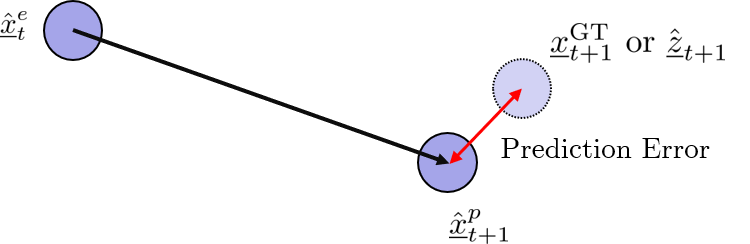
\includegraphics[width=0.6\textwidth]{figures/KF/prediction error.png}
\caption{Definition of the prediction error of a single track.}
\label{prediction error}
\end{figure}


For the whole dataset, the prediction error $E_{\mathrm{p}}$ is defined as the summation of the prediction error of all tracks dividing the number of tracks in the tracking result. The formula of the $E_{\mathrm{p}}$ is given as 
\begin{equation}
    E_{\mathrm{p}} = \frac{\sum_{i=1}^{n} d^{\mathrm{Err}}_{i}}{n}
\end{equation}


At the start and the end of the datasets, there are often some incomplete tracks that start or end in the middle of the tracking area. Because these tracks contain fewer measurements than the other tracks, the tracking accuracy can be also different. In order to reduce the effect of the incomplete tracks, the first and last ten tracks are not included in the calculation of the prediction error. In the optimization, our objection is to find the values of the prediction hyperparameters that minimize the prediction error $E_{\mathrm{p}}$ with the given dataset, as $\underset{\text{hyperparameters}}{\arg\max} E_{\mathrm{p}}(\mathrm{hyperparameters}, \textrm{dataset})$.


\subsection{Association Error}
\label{Association Error}

In the tracking process, each measurement comes from a certain particle. The association process constructs one-to-one correspondences between the tracks and the measurements in each timestep. When the correspondences are different from the real correspondences between particles and measurements, there are association errors. The association error contains errors of the first and second kind. We define the first kind of error as a track including the measurements which should belong to other tracks. An example is depicted in Figure \ref{asso err}b. An error belongs to the second kind of error when is that a measurement is assigned to a wrong track, as illustrated in Figure \ref{asso err}c \cite{pfaff2019multitarget}. 

The first and kind association accuracy rate $A_{a,1}$ and $A_{a,2}$ are defined respectively as the number of the correctly associated tracks or measurements dividing the number of tracks or measurements in the reference tracking result, as
\begin{equation}
    A_{a,1}=\frac{n_{\mathrm{tracks}}^{\mathrm{correct}}}{n_{\mathrm{tracks}}},\quad
    A_{a,2}=\frac{n_{\mathrm{measurement}}^{\mathrm{correct}}}{n_{\mathrm{measurement}}}.
\end{equation}
The harmonic mean association error rate $E_{a}=1-\frac{2A_{a,1}A_{a,2}}{A_{a,1}+A_{a,2}}$ is used in the following part for explaining the general accuracy of the association. The reference tracking result has no association error, and the association result is manually examined, as mentioned in Chapter 4.


\begin{figure}[htbp]
\centering
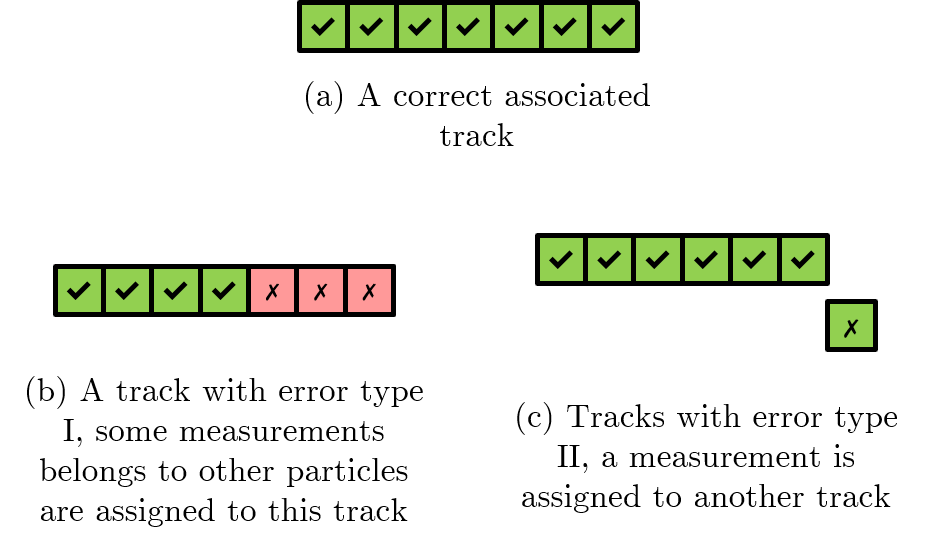
\includegraphics[width=0.7\textwidth]{figures/Asso/association error.png}
\caption{Illustrations for the two types of association errors. The color of the cells indicates the ID of the actual particle from which the measurement stems, adapted from \cite{pfaff2019multitarget}.}
\label{asso err}
\end{figure}

Association errors can be caused by different factors. For example, when two particles collide, the measurements from both particles can exchange to the tracks from another particle, as illustrated in Figure \ref{asso err2}a. Another example is that a particle is assigned to two separate tracks. It can occur when the particle is not observed in some frames, as depicted in Figure \ref{asso err2}b. But even if the measurements are continuous, this type of error can still happen when the prediction is too far away from the measurement or the association hyperparameters are chosen beyond the reasonable range, as shown in Figure \ref{asso err2}c. 

\begin{figure}[htbp]
\centering
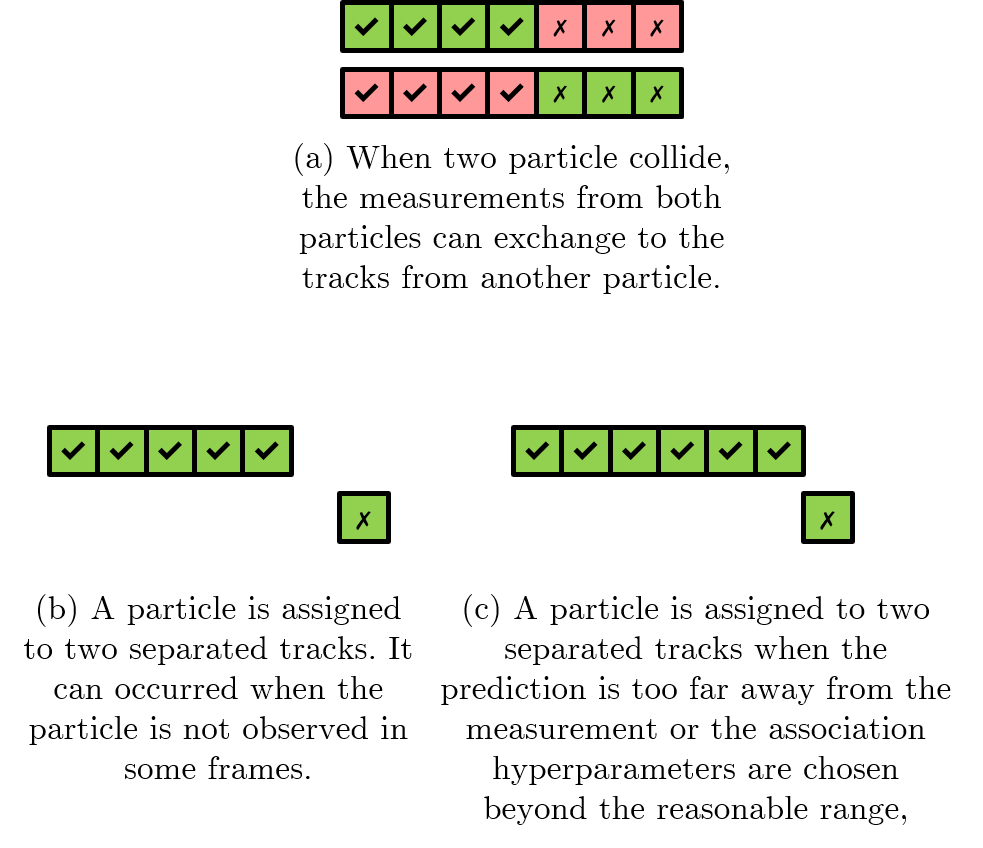
\includegraphics[width=0.7\textwidth]{figures/Asso/association error2.png}
\caption{Illustrations of some typical association errors, inspired from \cite{pfaff2019multitarget}.}
\label{asso err2}
\end{figure}

\section{Optimization of the Hyperparameters of Motion Prediction}  

% \textcolor{red}{added a introduction here. The loss function is also here}

In this section, we introduce the operations for the optimization of the prediction hyperparameters. First, the grid search is applied on the test dataset, for providing an initial knowledge of the effect of the hyperparameters. The hyperparameters and their range for the optimization are also determined with this step. Then, the optimized hyperparameters are obtained with the Bayesian optimization method. The validation method of Bayesian optimization is also introduced in this section. The loss function used in this section is the prediction error $E_{\mathrm{p}}$.

\subsection{Grid Search}

As mentioned in \Sec{gs}, grid search can give us the initial impression of the effect of each hyperparameter. These results can also prompt us for the selection and the range of the hyperparameters in the optimization. In this section, each hyperparameter for prediction was tested with the grid-search-like method. 

All the parameters were checked separately. To avoid the exploding number of searches, only 1-D and 2-D grid searches were performed, which means that only one or two hyperparameters were changed in each set of experiments, and the other hyperparameters remained as the default values. Some of the default values were set as constants, and the others were related to the initial velocity guess. The default values are listed in the Table \ref{defaultCV}, \ref{defaultCVA} and \ref{defaultasso1}. These values were also applied in the Bayesian optimization part for the not optimized hyperparameters.

The test data for the grid search are from the homogeneous material datasets. From each material, only one dataset with the reference result is selected for the grid

\begin{table}[htb] 
    \centering
    \caption{List of the default value of the hyperparameters for CV model.} 
    \begin{tabular}{ccc} 
    \toprule 
    Hyperparameters&Notation& Default value\\ 
    \midrule 
    \multirow{2}*{Initial velocity guess}&\multirow{2}*{$v_{0}$}&100 for homogeneous materials\\
     & & 65 for mixed materials\\
    Initial position variance&$S_{\mathrm{pos}}^{\mathrm{ini}}$&2000\\
    Initial velocity variance           &$S_{\mathrm{vel}}^{\mathrm{ini}}$&$v_{0}/6$\\
    Refined initial velocity variance   &$S_{\mathrm{vel}}^{\mathrm{ini, r}}$&1\\
    Measurement variance&$S^{\boldsymbol{v}}$&2000\\
    System noise variance &$S^{\boldsymbol{w}}$&1\\ 
    \bottomrule 
    \end{tabular} 
    \label{defaultCV}
\end{table}

\begin{table}[htb] 
    \centering
    \caption{List of the default value of the hyperparameters for CVA model.} 
    \begin{tabular}{ccc} 
    \toprule 
    Hyperparameters&Notation& Default value\\ 
    \midrule 
    \multirow{2}*{Initial velocity guess}&\multirow{2}*{$v_{0}$}&100 for homogeneous materials\\
     & & 65 for mixed materials\\
    Initial position variance           &$S_{\mathrm{pos}}^{\mathrm{ini}}$&2000\\
    Initial velocity variance           &$S_{\mathrm{vel}}^{\mathrm{ini}}$&$v_{0}/6$\\
    Refined initial velocity variance   &$S_{\mathrm{vel}}^{\mathrm{ini, r}}$&1\\
    Initial angle variance              &$S_{\mathrm{ang}}^{\mathrm{ini}}$&2\\
    Measurement position variance     &$S_{\mathrm{pos}}^{\boldsymbol{v}}$&2000\\
    Measurement velocity variance &$S_{\mathrm{vel}}^{\boldsymbol{v}}$&$v_{0}/30$\\
    Measurement angle variance      &$S_{\mathrm{ang}}^{\boldsymbol{v}}$&1\\
    Prediction position variance &$S_{\mathrm{pos}}^{\boldsymbol{w}}$&$v_{0}/6$\\
    Prediction velocity variance &$S_{\mathrm{vel}}^{\boldsymbol{w}}$&$v_{0}/60$\\
    Prediction angle variance   &$S_{\mathrm{ang}}^{\boldsymbol{w}}$&0.5\\
    \bottomrule 
    \end{tabular} 
    \label{defaultCVA}
\end{table}

\begin{table}[htb] 
    \centering
    \caption{List of the default value of the association hyperparameters for real materials.} 
    \begin{tabular}{ccc} 
    \toprule 
    Hyperparameters&Notation& Default value\\ 
    \midrule 
    Distance appear at start &$d_{\mathrm{as}}$&0.1\\
    Distance appear at middle &$d_{\mathrm{am}}$&1.5\\
    Distance disappear at end &$d_{\mathrm{de}}$&0.1\\
    Distance disappear at middle &$d_{\mathrm{dm}}$&1.5\\
    Distance no change &$d_{\mathrm{n}}$&0.1\\
    Starting phase coefficient&$l_{\mathrm{s}}$&1.3\\
    Ending phase coefficient&$l_{\mathrm{e}}$&0.5\\
    \bottomrule 
    \end{tabular} 
    \label{defaultasso1}
\end{table}

\FloatBarrier

% \textcolor{red}{added datasets and stepsize here}

search. In order to cover both the high and low values of the hyperparameters, the grid points for searching are set log-likely, as [1, 2, 5, 10, 20,..., 50000, 100000]. According to the default value of the hyperparameters, the search range for position variance is [1, 100000], and the range for other hyperparameters is [0.01, 1000]. 




\subsection{Bayesian Optimization}

% First is the setting of the Bayesian optimization, including parameters and some pre- and postprocedings aside of the optimization algorithm itself. These settings are also applied to the optimization of the real datasets.

% \subsection{Optimization Setting}
% \textcolor{red}{added the parameters for the optimization here}

In order to determine the optimized value of the hyperparameters of motion prediction, the Bayesian optimization method was applied for the optimization. In this part, only the most important hyperparameters were optimized. The hyperparameters for optimization were determined with the result of gird search, respectively the system noise variance $S^{\boldsymbol{w}}$ in the CV model and the prediction position variance $S_{\mathrm{pos}}^{\boldsymbol{w}}$ in the CVA model. The detailed selection process of the hyperparameters for optimization will be presented in the next chapter. In this section, ten datasets from each homogeneous material and all the three datasets from the mixture material were used as the data for the optimization. The objective function for optimization is the prediction error of each dataset.

The optimization was accomplished with the \textit{bayesopt} function in \textsc{Matlab}. The objective function was the prediction error in \Sec{Association Error}. The values of the important arguments for Bayesian optimization are presented in Table \ref{bayopt setting}. The argument \say{ExplorationRatio} is a parameter controlling the ratio of the exploiting and exploring, which have a similar effect with the exploration ratio in \Sec{bayopt intro}. \say{MaxObjectiveEvaluations} determines the iteration number of each optimization. The acquisition function used in the optimization is the expected improvement acquisition function with \textit{Per Second} and \textit{Plus} method. The other arguments remained as default in optimization. These settings applied to all datasets.

\begin{table}[htbp] 
    \centering
    \caption{Settings of the \textit{bayesopt} function.} 
    \begin{tabular}{cc} 
    \toprule 
    Arguments in the \textit{bayesopt} function&Value\\ 
    \midrule 
    \textquoteleft ExplorationRatio\textquoteright           &0.6\\
    \textquoteleft MaxObjectiveEvaluations\textquoteright    &20\\
    \textquoteleft AcquisitionFunctionName\textquoteright    &\textquoteleft expected-improvement-per-second-plus\textquoteright\\
    \bottomrule 
    \end{tabular} 
    \label{bayopt setting}
\end{table}



% \subsection{Clustering}


\section{Robust Range Determination of the Association Hyperparameters}

% \subsection{Robust Range of the Association Hyperparameters}
\label{Robust Range of the Association Hyperparameters}

Different from the hyperparameters of motion prediction, the association hyperparameters have no particular optimized value, but only a robust range. In this thesis, the robust range is defined as the range of the hyperparameters, with which the association error is zero. When the association hyperparameters are taken from this range, the association error will remain zero, even if under different values of the hyperparameters.

Take the association matrix in Figure \ref{asso example} as an example. In this matrix, the two measurements should be assigned to two existing tracks. The distance disappear and appear at middle are set both at 2. Under these circumstances, as long as the distance no change is lower than 3, the association can be correctly performed. Therefore, $[0,3]$ is recognized as the robust range of the hyperparameter distance no change.

\begin{figure}[htbp]
\centering
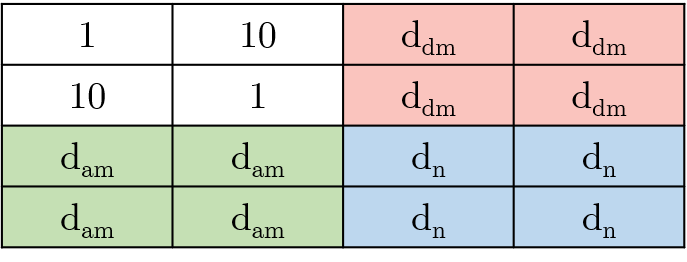
\includegraphics[width=0.4\textwidth]{figures/Asso/association matrix example.png}
\caption{An example of the association matrix.}
\label{asso example}
\end{figure}


\begin{figure}[htbp]
	\centering
	\begin{subfigure}[t]{0.5\textwidth}
		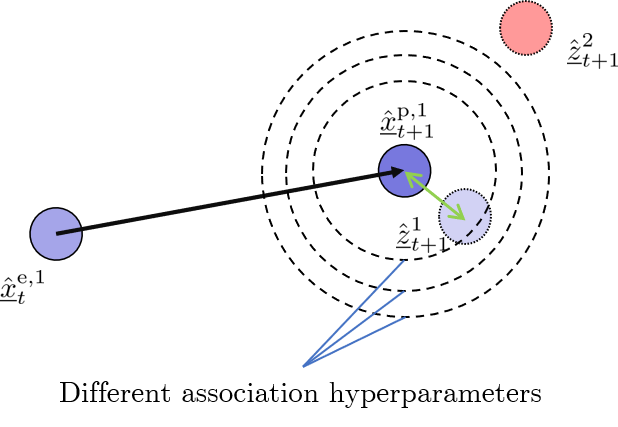
\includegraphics[width=\textwidth]{figures/Asso/robust range1.png}
		\caption{An association without error. The association hyperparameters are in the robust range.}
		\label{robust range1}
	\end{subfigure}
% 	\label{robust range1}
	% \hfill
	\vskip\baselineskip
	
	\begin{subfigure}[t]{0.4\textwidth}
		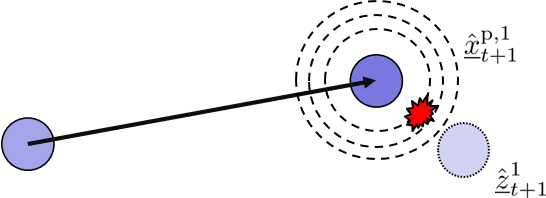
\includegraphics[width=\textwidth]{figures/Asso/robust range2.png}
		\caption{An association error occurred because the bound of association is too low.}
		\label{robust range2}
	\end{subfigure}
	\quad
	\begin{subfigure}[t]{0.3\textwidth}
		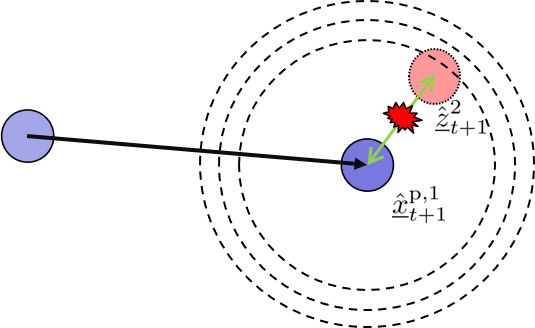
\includegraphics[width=\textwidth]{figures/Asso/robust range3.png}
		\caption{An association error occurred because the bound of association is too high.}
		\label{robust range3}
	\end{subfigure}
% 	\begin{subfigure}[t]{0.4\textwidth}
% 		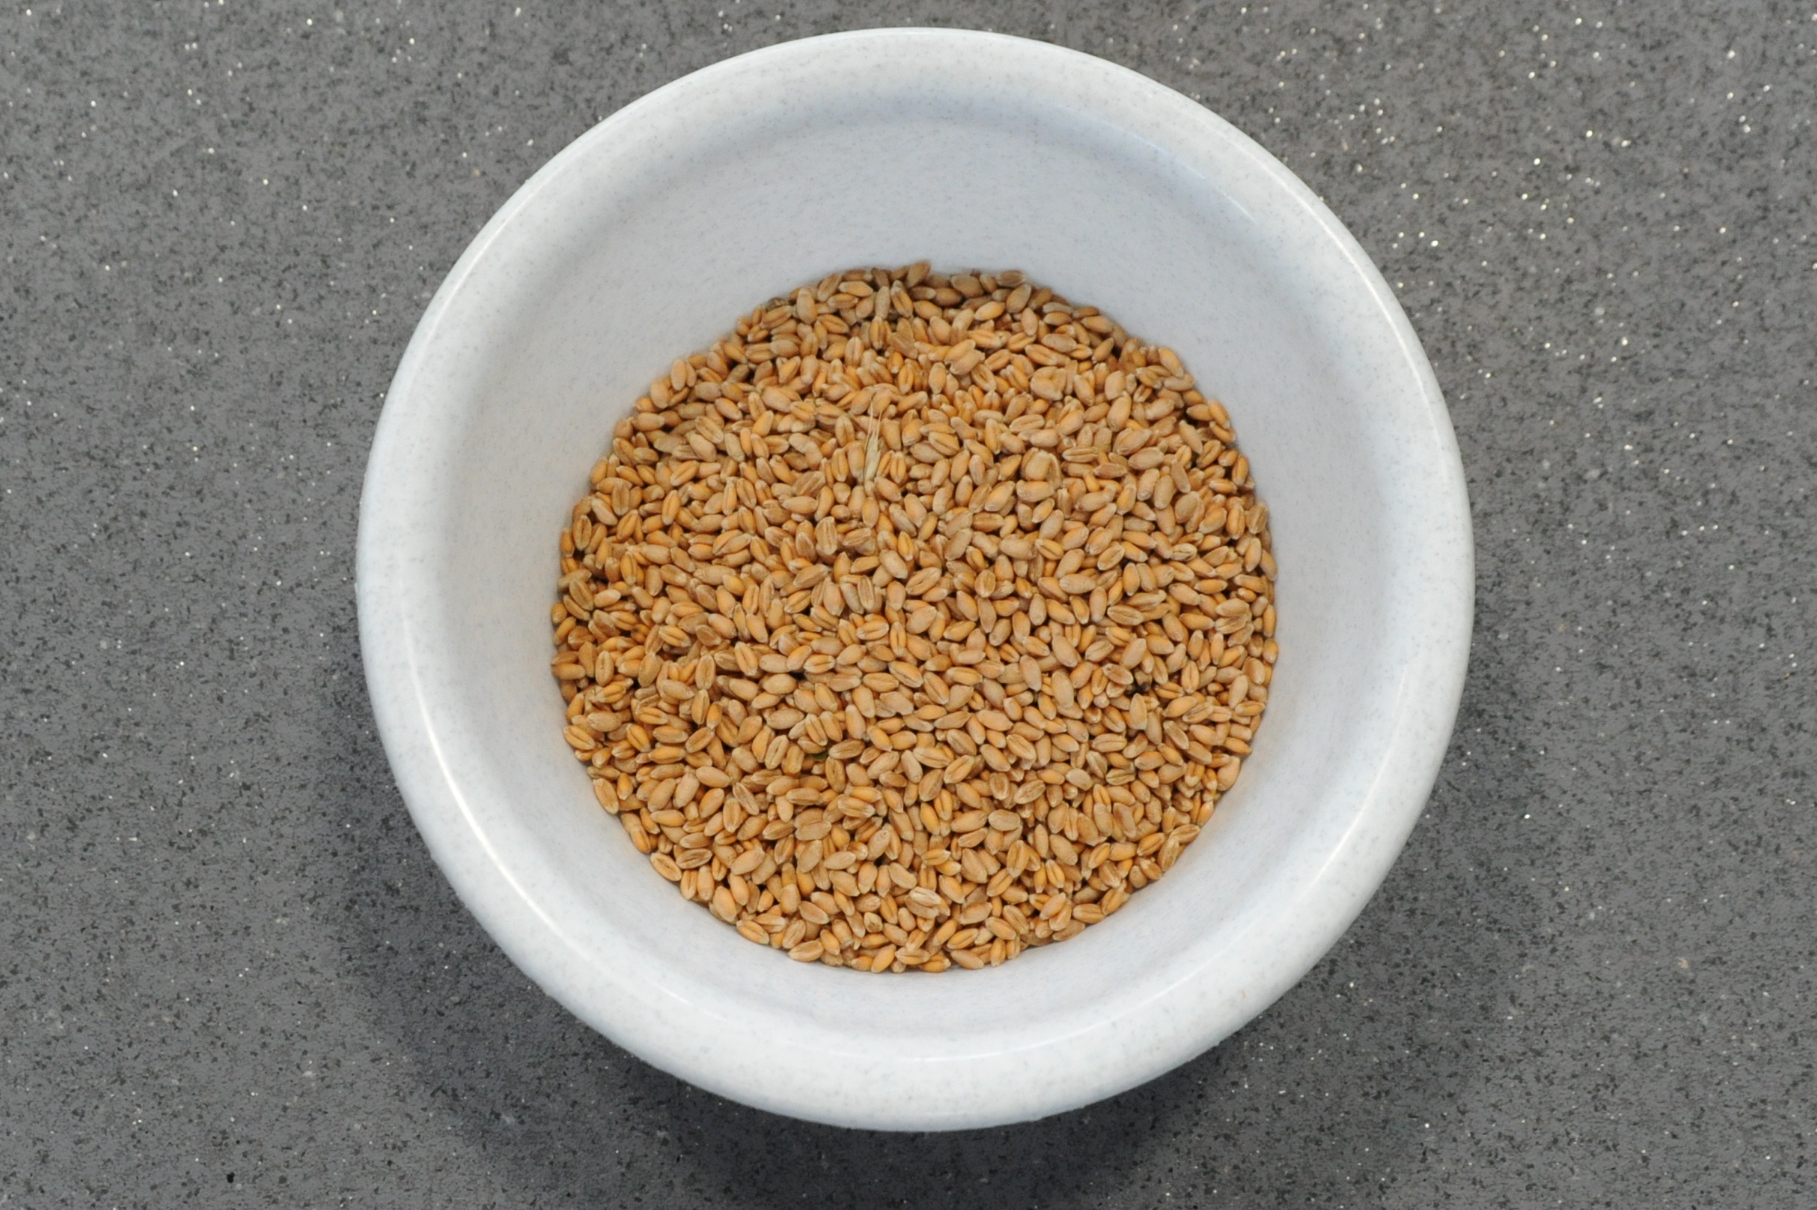
\includegraphics[width=\textwidth]{WeizenCropped2}
% 		\caption{Wheat grains}
% 	\end{subfigure}
	\caption{The effect of the value of the association parameters. When the association hyperparameters are in the robust range, as illustrated in Figure (a), the association can be performed without error, even if the values of the hyperparameters are different, as shown with the different radius of the black dashed circle. However, when the hyperparameters go beyond the robust range, the association error occurs, as illustrated in Figure (b) and (c).}
	\label{robust range}
\end{figure}


In the following part of this thesis, the robust range of the distance-like penalty terms in the association matrix are examined with 1-D grid search and SVM. Because the coefficients for the range of different tracking phases can be directly derived from the analysis of the tracking area, these coefficients are discussed separately.


\subsection{Grid Search}
With grid search, we can figure out the effect of each association hyperparameter on the association error and get a rough estimation of the robust range of each hyperparameter. The grid search is performed with the CVA model in this section where only one association hyperparameter is changed in a set of searches, and the other hyperparameters remain as default values, as shown in Table \ref{defaultCVA2} and \ref{defaultasso2}. The test data for the grid search are from the DEM datasets. The search range is [0, 0.03] with a step size of 0.001.




\begin{table}[htbp] 
    \centering
    \caption{List of the default value of the prediction hyperparameters for DEM datasets.} 
    \begin{tabular}{ccc} 
    \toprule 
    Hyperparameters&Notation& Default value\\ 
    \midrule 
    Initial velocity guess              &$v_{0}$&0.01\\
    Initial position variance           &$S_{\mathrm{pos}}^{\mathrm{ini}}$&$v_{0}/15$\\
    Initial velocity variance           &$S_{\mathrm{vel}}^{\mathrm{ini}}$&$v_{0}/6$\\
    Refined initial velocity variance   &$S_{\mathrm{vel}}^{\mathrm{ini, r}}$&1\\
    Initial angle variance              &$S_{\mathrm{ang}}^{\mathrm{ini}}$&2\\
    Measurement position variance       &$S_{\mathrm{pos}}^{\boldsymbol{v}}$&$v_{0}/15$\\
    Measurement velocity variance       &$S_{\mathrm{vel}}^{\boldsymbol{v}}$&$v_{0}/30$\\
    Measurement angle variance          &$S_{\mathrm{ang}}^{\boldsymbol{v}}$&1\\
    Prediction position variance        &$S_{\mathrm{pos}}^{\boldsymbol{w}}$&$v_{0}/6$\\
    Prediction velocity variance        &$S_{\mathrm{vel}}^{\boldsymbol{w}}$&$v_{0}/60$\\
    Prediction angle variance           &$S_{\mathrm{ang}}^{\boldsymbol{w}}$&0.5\\
    \bottomrule 
    \end{tabular} 
    \label{defaultCVA2}
\end{table}


\begin{table}[htbp] 
    \centering
    \caption{List of the default value of the association hyperparameters for DEM datasets.} 
    \begin{tabular}{ccc} 
    \toprule 
    Hyperparameters&Notation& Default value\\ 
    \midrule 
    Distance appear at start        &$d_{\mathrm{as}}$&0.001\\
    Distance appear at middle       &$d_{\mathrm{am}}$&0.03\\
    Distance disappear at end       &$d_{\mathrm{de}}$&0.001\\
    Distance disappear at middle    &$d_{\mathrm{dm}}$&0.03\\
    Distance no change              &$d_{\mathrm{n}}$&0.0001\\
    Starting phase coefficient      &$l_{\mathrm{s}}$&1.3\\
    Ending phase coefficient        &$l_{\mathrm{e}}$&0.5\\
    \bottomrule 
    \end{tabular} 
    \label{defaultasso2}
\end{table}


\subsection{Data and Setting for the SVM training}
\label{training data svm}

% \textcolor{red}{added more detailed info}
In this section, some SVMs that can give us information about the robust range in higher dimensional hyperparameter spaces are trained. The SVMs can also provide us a model to estimate whether a given set of values of the association hyperparameters are in the robust range. 

The data for the training of the SVMs were generated with the \textit{TrackSort} Algorithm and the DEM dataset. The tracking results were compared with the reference dataset to determine the association error rate. Then these results were binary labeled by whether the association error occurs. The label for each tracking result was recorded along with the association hyperparameters. These hyperparameter tracking error pairs were used as the training dataset of the SVM. 

The training of SVM was performed with 2-D and 5-D training datasets. Each 2-D dataset, where only two hyperparameters were changed and the other hyperparameters remained as default, includes 100 data points for training. The 2-D datasets include each combination of the hyperparameters. The 5-D dataset, where all the five distance-like penalty terms are changed, includes 10,000 data points. The SVM is trained with 10-fold training, where the dataset is divided into 10 folds in equal size. In each training, nine folds of the data points will be the training data and the left fold serves as the test set. The final model is taken from the best result in all 10 training results. All the data were generated with the CVA model, and the prediction hyperparameters for these datasets are shown in Table \ref{defaultCVA2}. The values for the unchanged association hyperparameters with DEM datasets are presented in Table \ref{defaultasso2}. 
% The initial velocity guess for the DEM dataset is set as 0.01.


% \subsection{Setting of the SVM Training}

The training of the SVM was accomplished with the \textit{fitcsvm} function in \textsc{Matlab}. The objective function is the prediction error in \Sec{Association Error}. The values of the important arguments for Bayesian optimization are presented in Table \ref{bayopt setting}. We used the RBF kernel for the SVM. The hyperparameters for the SVM including the penalty factor $c$ and the kernel size $\sigma$ were automatically optimized with Bayesian optimization. The other arguments remained as default. For the 5-D SVMs, we used 10-fold cross-validation. The SVMs provide us classifiers of the hyperparameters that output whether the association error is zero with the given set of hyperparameters. The decision boundary of the SVMs is considered as the robust range of the hyperparameters.

\begin{table}[htbp] 
    \centering
    \caption{Settings of the \textit{fitcsvm} function.} 
    \begin{tabular}{cc} 
    \toprule 
    Arguments in the \textit{fitcsvm} function&Value\\ 
    \midrule 
    \textquoteleft KernelFunction\textquoteright             &'rbf'\\
    \textquoteleft OptimizeHyperparameters\textquoteright    &'auto'\\
    \multirow{2}*{\textquoteleft HyperparameterOptimizationOptions\textquoteright}&struct(\textquoteleft AcquisitionFunctionName',\\
     & \textquoteleft expected-improvement-plus'))\\
    \textquoteleft KFold\textquoteright&                  10\\
    \bottomrule 
    \end{tabular} 
    \label{svm setting}
\end{table}

 